\documentclass[a4paper,11pt]{jsarticle}


% 数式
\usepackage{amsmath,amsfonts,amssymb}
\usepackage{bm}
% 画像
\usepackage[dvipdfmx]{graphicx}
\usepackage[dvipdfmx]{color}
\usepackage{siunitx}
\usepackage{wrapfig}
\usepackage{cases}
\usepackage{dcolumn}
\makeatletter
\newcommand{\figcaption}[1]{\def\@captype{figure}\caption{#1}}
\newcommand{\tblcaption}[1]{\def\@captype{table}\caption{#1}}
\makeatother

\usepackage{listings,jvlisting}
\lstset{
basicstyle={\ttfamily},
identifierstyle={\small},
commentstyle={\smallitshape},
keywordstyle={\small\bfseries},
ndkeywordstyle={\small},
stringstyle={\small\ttfamily},
frame={tb},
breaklines=true,
columns=[l]{fullflexible},
numbers=left,
xrightmargin=0zw,
xleftmargin=3zw,
numberstyle={\scriptsize},
stepnumber=1,
numbersep=1zw,
lineskip=-0.5ex
}

% for next page in the middle of eq
\allowdisplaybreaks[1]

\begin{document}

\title{
  端点と2重振り子の全体の重心を結ぶ線分の角速度と
  2重振り子の各セグメントの重心を結ぶ線分の角速度の関係
}
\author{平林広}
\date{\today}
\maketitle

\begin{figure}[h]
  \centering
  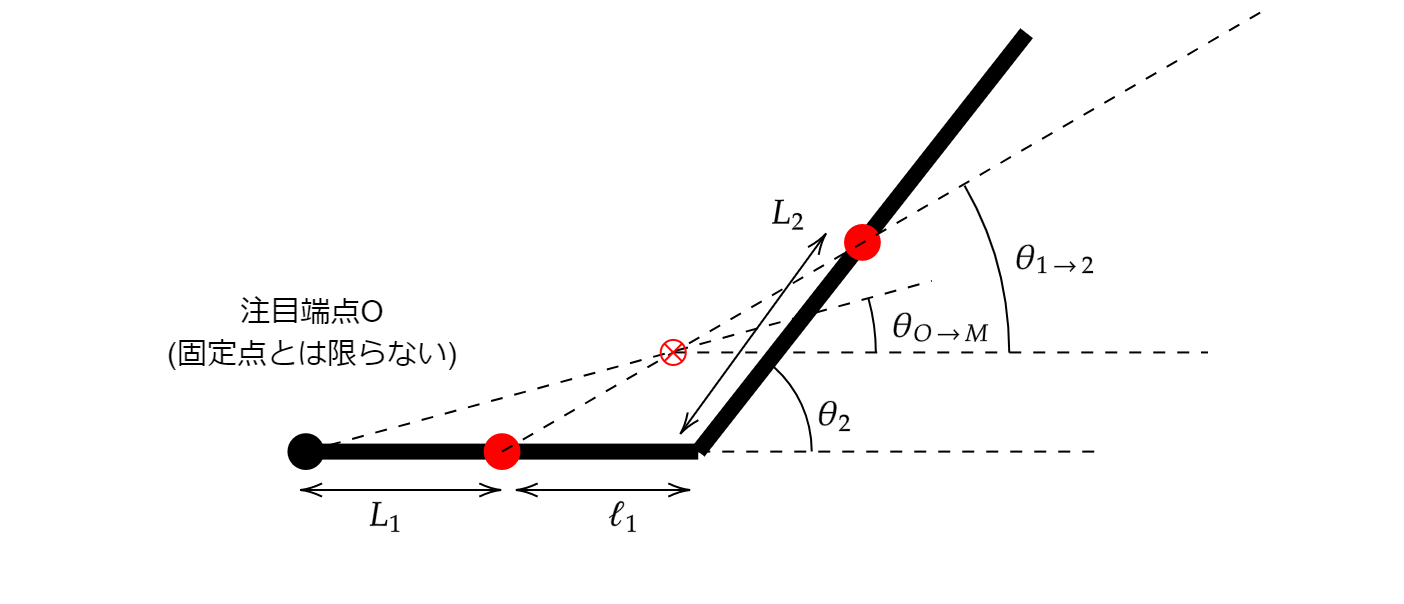
\includegraphics[width = 0.95\textwidth]{conf.png}
  \caption{文字設定}
  \label{conf.png}
\end{figure}

この文章の目的は
$\dot\theta_{O\rightarrow M} - \dot\theta_{1\rightarrow 2}$が
$\dot\theta_2$に対して比例関係であることと、
\begin{gather}
  \dot\theta_{O\rightarrow M} - \dot\theta_{1\rightarrow 2}
  = A \dot\theta_2
\end{gather}
としたときに比例定数$A$に関して$A<0$であることを証明することを目的とする。

セグメント1に対する相対座標を考える。
相対座標の原点を注目端点$\mathbf{O}$とし、
相対座標の回転の原点(軸ではなく、0度の方向)をセグメント1の方向とする。
回転座標系を考えると
コリオリの力など解釈が難しい項が出てくるが、
今回は速度の次元までしか微分しないために問題ない。

また、Millard 2019. の股関節を模し、
$|\theta_2|<90\,^\circ$とする。

全体の重心の位置ベクトルは
\begin{gather*}
  \left(
    \begin{gathered}
      \frac{M_1L_1 + M_2\left(L_1+\ell_1+L_2\cos\theta_2\right)}{M_1+M_2}
      \\
      \frac{M_1\cdot 0 + M_2L_2\sin\theta_2}{M_1+M_2}
    \end{gathered}
  \right)
  =
  \left(
    \begin{gathered}
      L_1 + \frac{M_2\left(\ell_1+L_2\cos\theta_2\right)}{M_1+M_2}
      \\
      \frac{M_1\cdot 0 + M_2L_2\sin\theta_2}{M_1+M_2}
    \end{gathered}
  \right)
\end{gather*}
と表される。
ゆえに2重振り子を単振り子に近似するための角度
$\theta_{O\rightarrow M}, \theta_{1\rightarrow 2}$に関して
\begin{align*}
  &\tan\theta_{O\rightarrow M}
  =\frac{
    M_2L_2\sin\theta_2
  }{
    (M_1+M_2)L_1 + M_2\left(\ell_1+L_2\cos\theta_2\right)
  }
  &=&\frac{L_2\sin\theta_2}{\frac{M_1+M_2}{M_1}L_1 + \ell_1 + L_2\cos\theta_2}
  \\
  \\
  &\tan\theta_{1\rightarrow 2}
  &=&\frac{
    L_2\sin\theta_2
  }{
    \ell_1+L_2\cos\theta_2
  }
\end{align*}
が成り立つ。
$|\theta_2|<90\,^\circ$より$\cos\theta_2>0\,\Rightarrow L_2\cos\theta_2>0$なので
\begin{align*}
  \theta_{O\rightarrow M}
  &= \arctan\left(\frac{L_2\sin\theta_2}{\frac{M_1+M_2}{M_1}L_1 + \ell_1 + L_2\cos\theta_2}\right)
  \\
  \theta_{1\rightarrow 2}
  &= \arctan
  \left(\frac{ L_2\sin\theta_2}{\ell_1+L_2\cos\theta_2} \right)
\end{align*}
が成り立つ。

まず$\dot\theta_{1\rightarrow 2}$から求める。
というのも、$\theta_{O\rightarrow M}, \theta_{1\rightarrow 2}$
は
$\frac{M_1+M_2}{M_1}L_1+\ell_1 \leftrightarrow \ell_1$という関係だから、
$\dot\theta_{1\rightarrow 2}$が求まれば
$\dot\theta_{O\rightarrow M}$は簡単に求まる。
$\frac{d}{dt}\arctan t = \frac{1}{1+t^2}$であることから、
\begin{align*}
  \dot\theta_{1\rightarrow 2}
  &= \frac{d}{dt}
  \arctan
  \left(\frac{ L_2\sin\theta_2}{\ell_1+L_2\cos\theta_2} \right)
  \\
  &=\frac{1}{1+\left(\frac{ L_2\sin\theta_2}{\ell_1+L_2\cos\theta_2} \right)^2}
  \cdot
  \frac{d}{dt}\left(
    \frac{L_2\sin\theta_2}{\ell_1+L_2\cos\theta_2}
  \right)
  \\
  &= \frac{1}{1+\left(\frac{ L_2\sin\theta_2}{\ell_1+L_2\cos\theta_2} \right)^2}
  \cdot
  \frac{
    L_2\cos\theta_2\cdot (\ell_1+L_2\cos\theta_2) - L_2\sin\theta_2\cdot L_2(-\sin\theta_2)
  }{
    (\ell_1+L_2\cos\theta_2)^2
  }
  \frac{d}{dt}\theta_2
  \\
  &= \frac{1}{1+\left(\frac{ L_2\sin\theta_2}{\ell_1+L_2\cos\theta_2} \right)^2}
  \cdot
  \frac{
    \ell_1L_2\cos\theta_2 + L_2{}^2\cos^2\theta_2 + L_2{}^2\sin^2\theta_2
  }{
    (\ell_1+L_2\cos\theta_2)^2
  }
  \dot\theta_2
  \\
  &= \frac{
    \ell_1L_2\cos\theta_2 + L_2{}^2
  }{
    (\ell_1+L_2\cos\theta_2)^2 + L_2{}^2\sin^2\theta_2
  }
  \dot\theta_2
  \\
  &= \frac{
    \ell_1\cos\theta_2 + L_2
  }{
    \ell_1{}^2 + 2\ell_1L_2\cos\theta_2 + L_2{}^2
  }
  L_2
  \dot\theta_2
\end{align*}
ここで
\begin{gather*}
  f(x) = \frac{
    x\cos\theta_2 + L_2
  }{
    x^2 + 2xL_2\cos\theta_2 + L_2{}^2
  }
  L_2
\end{gather*}
とすると、
\begin{gather*}
  \dot\theta_{O\rightarrow M} = f\left(\ell_1 + \frac{M_1+M_2}{M_1}L_1\right)\dot\theta_2
  \\
  \dot\theta_{1\rightarrow 2} = f(\ell_1)\dot\theta_2
\end{gather*}
と簡潔に書け、
\begin{gather*}
  \dot\theta_{O\rightarrow M} - \dot\theta_{1\rightarrow 2}
  = \left[
    f\left(\ell_1 + \frac{M_1+M_2}{M_1}L_1\right) - f(\ell_1)
  \right]\dot\theta_2
  \\
  \Rightarrow
  A = f\left(\ell_1 + \frac{M_1+M_2}{M_1}L_1\right) - f(\ell_1)
\end{gather*}
であることが分かる。

ここで
$x>0$における$f(x)$の単調減少を示すことで、
$A<0$が証明できる。
\begin{align*}
  f' (x)
  &= \frac{
    \begin{aligned}
      \cos\theta_2 &\cdot (x{}^2 + 2xL_2\cos\theta_2 + L_2{}^2)
      \\
      &- (x\cos\theta_2 + L_2)\cdot (2x + 2L_2\cos\theta_2)
    \end{aligned}
  }{
    (x{}^2 + 2xL_2\cos\theta_2 + L_2{}^2)^2
  }
  L_2
  \\
  \\
  &= \frac{
    \begin{aligned}
      &x\cos\theta_2 
      &+& 2xL_2\cos^2\theta_2 
      &&
      &+& L_2{}^2\cos\theta_2
      \\
      -\Big(
        &2x{}^2\cos\theta_2 
        &+& 2xL_2\cos^2\theta_2
        &+& 2xL_2
        &+& 2L_2{}^2\cos\theta_2
      \Big)
    \end{aligned}
  }{
    (x{}^2 + 2xL_2\cos\theta_2 + L_2{}^2)^2
  }
  \\
  \\
  &=-\frac{
    x{}^2\cos\theta_2 + 2xL_2 + L_2{}^2\cos\theta_2
  }{
    (x{}^2 + 2xL_2\cos\theta_2 + L_2{}^2)^2
  }
  \\
  \\
  &= -\frac{
    \Bigl[(x{}^2 + L_2{}^2)\cos\theta_2 + 2xL_2\Bigr]
  }{
    (x{}^2 + 2xL_2\cos\theta_2 + L_2{}^2)^2
  }
  < 0 \quad (\because \cos\theta_2 > 0, \, x > 0, \, L_2 > 0).
\end{align*}
ゆえに
$x>0$において$f(x)$は単調減少するので
$\ell_1 + \frac{M_1+M_2}{M_1}L_1 > \ell_1 > 0$より
\begin{gather*}
  f\left(\ell_1 + \frac{M_1+M_2}{M_1}L_1\right) < f(\ell_1)
  \\
  \Rightarrow
  A = f\left(\ell_1 + \frac{M_1+M_2}{M_1}L_1\right) - f(\ell_1) < 0
\end{gather*}
が示された。

\end{document}